Un'ultima analisi effettuata è stata riguardo lo stato degli agenti durante il processo di esplorazione della mappa.
In particolare, si è studiato per ogni \textit{step} di una simulazione il numero di agenti che fossero nei seguenti stati:
\begin{itemize}
	\item esplorazione di una cella;
	\item movimento verso una cella;
	\item rilascio un ripetitore;
	\item scelta della prossima cella obiettivo o attesa dell'aggiunta di celle obiettivo.
\end{itemize}
Per raccogliere tali dati, è stata effettuata una singola simulazione su due mappe particolari generate \textit{ad hoc} e 5 mappe casual che non presentassero casi patologici.
Tutte le mappe sono di dimensione 30$\times$30, per questioni di tempo richiesto dalle singole simulazioni, $\alpha$ e $\gamma$ assumono valori pari ai valori indotti dal processo di ottimizzazione (Sezione \ref{sec:psoResults}), il raggio di percezione pari a 6 celle e quello dei ripetitori pari a 3 celle.
Inoltre, sono stati utilizzati 6 robot e i feriti potevano segnalare la loro presenza.\\
Le prima delle due mappe particolari rappresenta una situazione che vuole simulare la presenza di un ponte, ovvero si può considerare la mappa divisa in due parti che sono unite solo da una piccola porzione di terra attraversabile.
La seconda è una mappa che presenta delle zone non raggiungibili, non visibili e, quindi, non esplorabili.

I risultati raccolti sono riportati in Figura \ref{fig:status}; si noti che per rendere i dati leggibili sono stati calcolati 100 intervalli in cui suddividere i dati e questi ultimi sono stati aggregati all'interno di ogni intervallo. Per questo motivo in colore si notano le medie e in nero le relative \textit{errorbar}.
Dai grafici, si può dedurre come la maggior parte dei robot siano quasi sempre impegnati nell'esplorazione e passano poco tempo nelle altre fasi. Questo indica che i robot tendono sempre a scegliere le celle più economiche da raggiungere (poiché il valore del parametro $\alpha$ è elevato) e che passano la maggior parte del tempo a esplorare le celle.
Se così non fosse, ci sarebbe un numero medio di robot minore in fase di esplorazione.
Si può, infine, notare come la fase di rilascio dei ripetitori sia un'attività in cui tipicamente solo uno dei robot è impegnato, indicando quindi che la costruzione della rete \textit{mesh} non sia un collo di bottiglia che aumenta significativamente i tempi di esplorazione del territorio.
Infine, si faccia riferimento all'Appendice \ref{apx:status} per i grafici non qui rappresentati.

\begin{figure}
	\begin{tabular}{cc}
		\subfloat[Stato dei robot durante l'esplorazione della mappa con il ponte.]{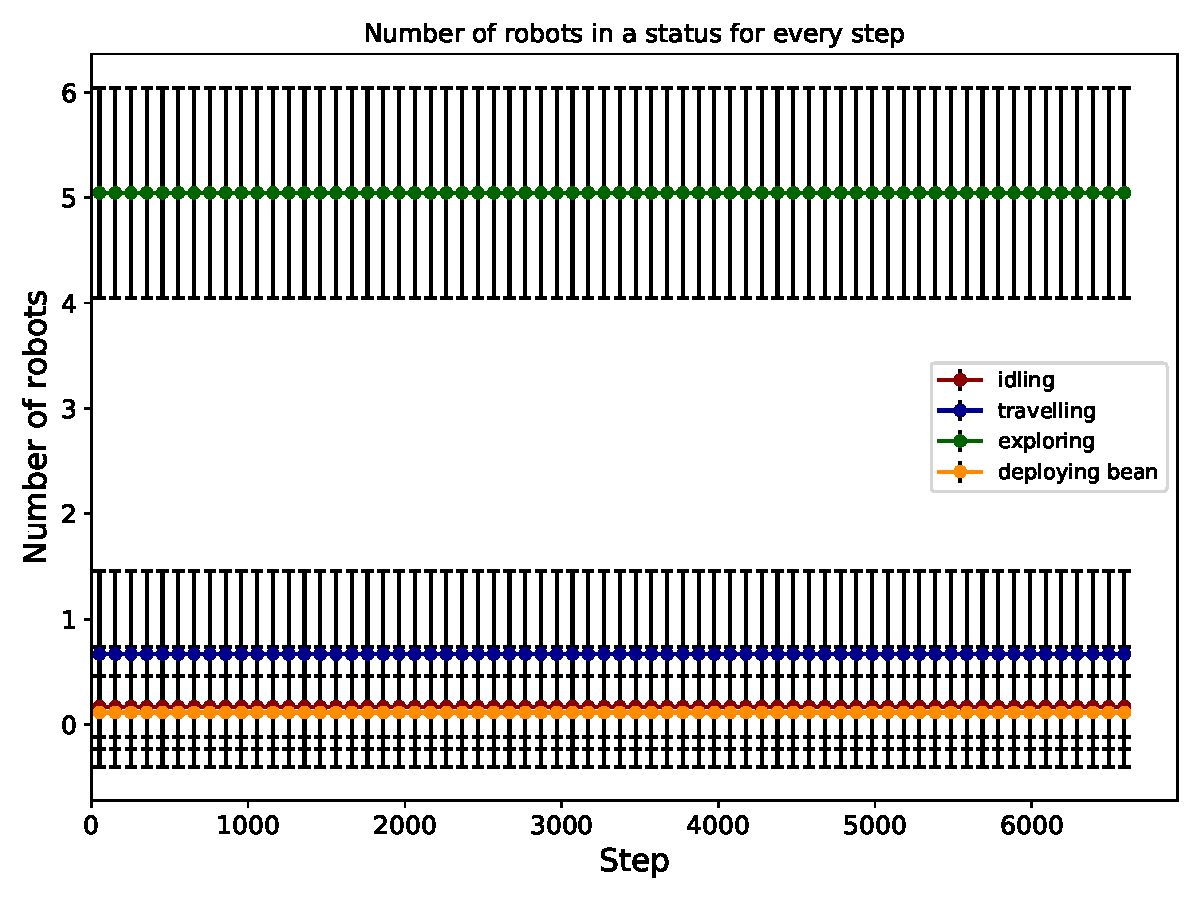
\includegraphics[width = .5\textwidth]{images/status_results/bridge_sim0}} &
		\subfloat[Stato dei robot durante l'esplorazione della mappa con zone non raggiungibili.]{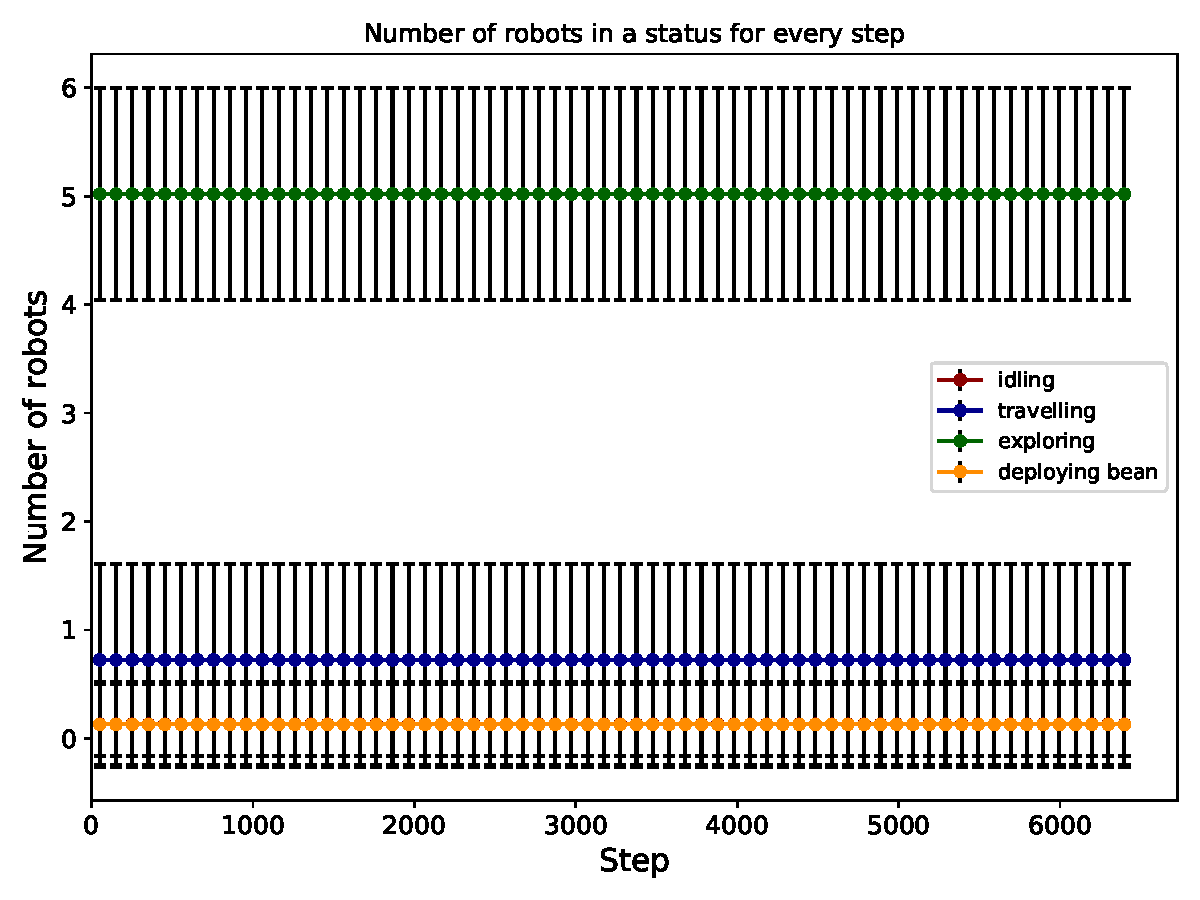
\includegraphics[width = .5\textwidth]{images/status_results/buildings_sim0}}\\
		\subfloat[Stato dei robot durante l'esplorazione della mappa generata casualmente numero 2.]{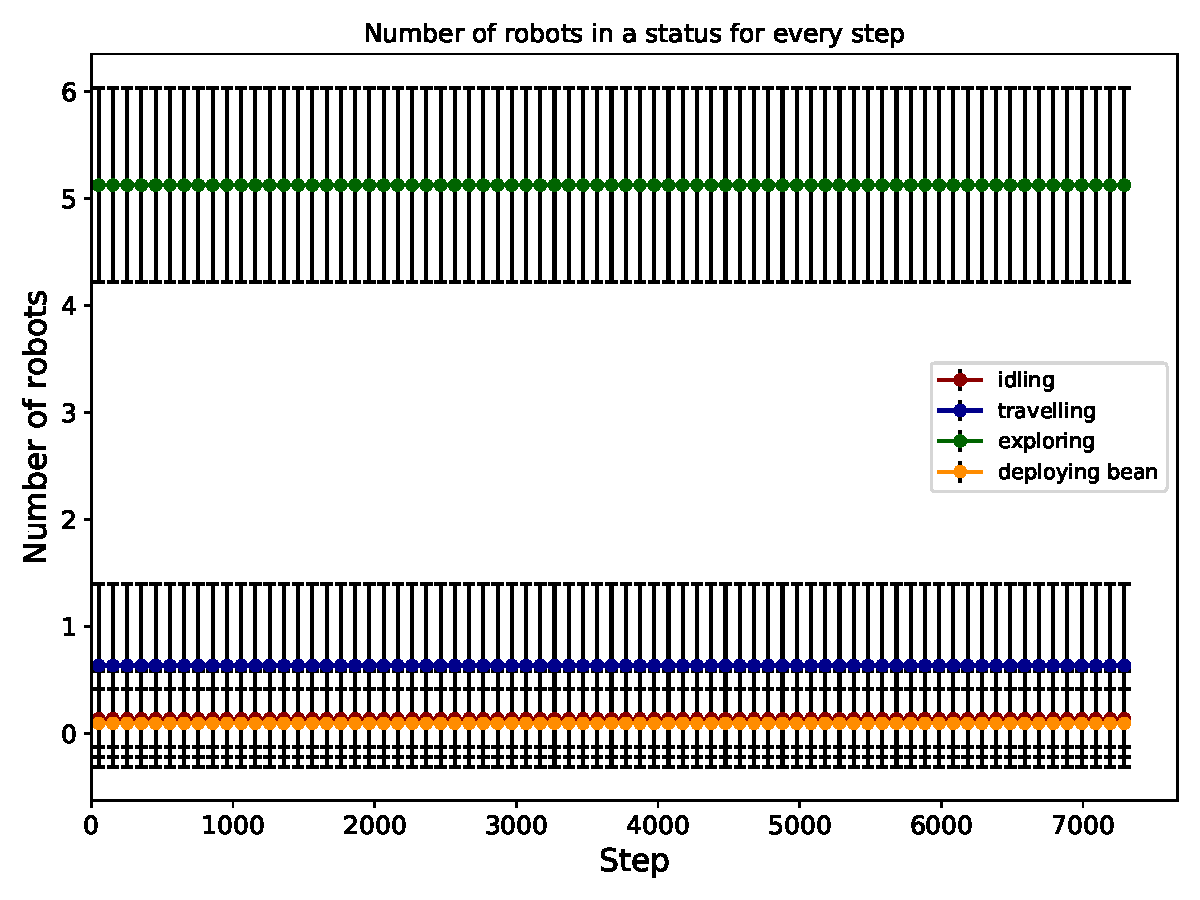
\includegraphics[width = .5\textwidth]{images/status_results/random2_sim0}} &
		\subfloat[Stato dei robot durante l'esplorazione della mappa generata casualmente numero 5.]{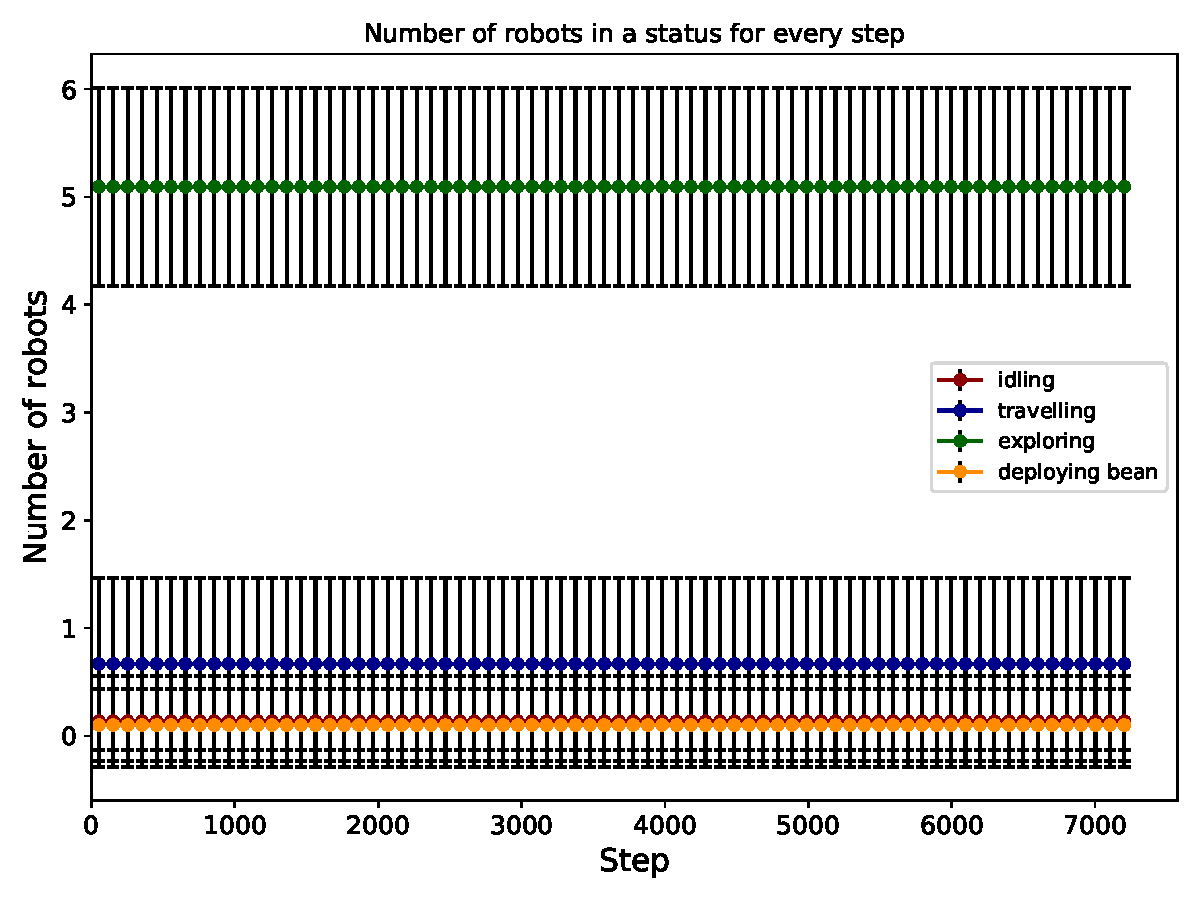
\includegraphics[width = .5\textwidth]{images/status_results/random5_sim0}}\\
	\end{tabular}
	\caption{Sull'asse delle \textit{x} si trova il tempo, in termini di \textit{step}, impiegato per l'esplorazione della mappa, mentre sull'asse delle \textit{y} il numero di agenti in un determinato stato. Si noti che i dati sono stati raggruppati per formare 100 \textit{bin} in modo da rendere leggibile il grafico; di conseguenza, in colore si trovano le medie e le \textit{errorbar} rappresentano le devizioni standard rispeto alla media.}
	\label{fig:status}
\end{figure}